\section*{Usage Notes}
%%Brief instructions that may help other researchers reuse these dataset.
%%This is an optional section, but strongly encouraged when helpful
%%to readers. This may include discussion of software packages that
%%are suitable for analyzing the assay data files, suggested downstream
%%processing steps (e.g. normalization, etc.), or tips for integrating
%%or comparing this with other datasets. If needed, authors are encouraged
%%to provide code, programs, or data processing workflows when they may help 
%%others analyse the data. We encourage authors to archive related code in 
%%a DOI-issuing archive when possible, but code may also be supplied as 
%%supplementary information files. 
%%
%%For studies involving privacy or safety controls on public access
%%to the data, this section should describe in detail these controls,
%%including how authors can apply to access the data, and what criteria
%%will be used to determine who may access the data, and any limitations
%%on data use.
Standartox can either be accessed through the APP or the API together with the R-package standartox. Both access pathways allow for the same filters and aggregation methods (Table \ref{tab:app-parameters} to be applied on the data. In the former the user can download the resulting data sets as a comma-separated values file whereas in the latter the user can directly load them in R. The user can choose among different parameters to filter and aggregate the test data accordingly \ref{tab:app-parameters}. The user can filter for compound-specific filters, including the CAS number, the concentration type (e.g. Active Ingredient, Formulation), the chemical class (e.g. Insecticides, Metals) and taxon-specific filters, including common taxonomic groups (e.g. Daphniidae, Algae), the habitat (e.g. freshwater) and the regional occurrence (e.g. Europe, Asia) of the organisms. Furthermore, the user can refine the results to specific test durations (in hours), effect groups (e.g. Mortaliy, Population, Growth) and endpoints (EC\textsubscript{50}, EC\textsubscript{10}, LOEC or NOEC).  As aggregates the user can choose the minimum, the maximum, the median, the geometric mean or the arithmetic mean. All the steps described in this section are selectable in the GUI and are executed at each click by the application. The drop down menu `Download data` allows to download a filtered data set as well as an aggregated data set.

Percentage values next to inputs show the proportion of the respective option (e.g. \textit{Active Ingredient - 43\%} indicates that 43\% of the data are Active Ingredients).

\subsection*{R package}
The R-package standartox consists of the two functions stx\_catalog() and stx\_query(). The former allows the retrieval of a catalog of possible parameters that can be used as an input for the latter. stx\_query() fetches the toxicity values from the data base and returns them as a R list object (compare Code \ref{listing:standartox-example}).

\begin{lstlisting}[
    caption = {standartox R-package code} example,
    label = {listing:standartox-example}]
# install
install.packages('remotes')
remotes::install_github('andschar/standartox') # package not yet on CRAN
# retrieve catalog    
require(standartox)
catal = stx_catalog()
# retrieve data
l = stx_query(cas = '1071-83-6',
                endpoint = 'XX50',
                taxa = 'Oncorhynchus',
                duration = c(24, 120))
\end{lstlisting}

Standartox is designed to support CRA. With an increased amount of available ecotoxicological test data, it becomes fundamental to provide and distribute such information in reasonable formats, meaning accessible for humans as well as machines. Currently CRA often relies on test results of a few, well tested standard organism, such as \textit{Daphnia magna}, \textit{Pimephales promelas}, \textit{Selenastrum capricornutum}, although researchers have conducted experiments on a much greater variety of organisms (e.g. the 926,108 test results collected in the EPA ECOTOX data base). In order to locate ecotoxicological test data, researchers can rely on individual test results reported in publications <CITE>, on compiled and published data sets \citep{malaj_organic_2014} or on data bases such as the Pesticide Property Data Base (PPDB) \citep{lewis_international_2016}. Each data source has its limitations though: Collecting toxicity information from individual publications is laborious and using already compiled data from publications or data bases is often limited to a specific groups of chemicals, such as pesticides, biozides etc. Standartox, making use of the EPA ECOTOX, the largest publicly available collection of ecotoxicological test results, aims to facilitate the data retrieval process by providing adequate aggregates (EC\textsubscript{50}, NOEC, LOEC) of the tests results. These are then used for the calculation of SSDs, TUs or other risk indicators. SSDs try to extrapolate effects of chemicals towards organisms from species to a community level by fitting a statistical distribution to toxicity test results on organisms of different trophic levels in order to derive concentrations at which a specific fraction of organisms are effected (often at 5\% - HC\textsubscript{5} \citep{posthuma_species_2002}. Figure \ref{fig:ssd-isoproturon} shows an example of a SSD and the derived HC\textsubscript{5} value (red dassed line) created for the herbicide Isoproturon. TUs are another indicator of effects of chemicals on organisms. They are calculated by dividing a measured concentration (c) by an EC\textsubscript{50} value (cf. Equation \ref{eq:tu}).

\begin{equation}
    TU_i = \frac{c_i}{\ecfifty}
    \label{eq:tu}
\end{equation}

\begin{figure}[h!]
    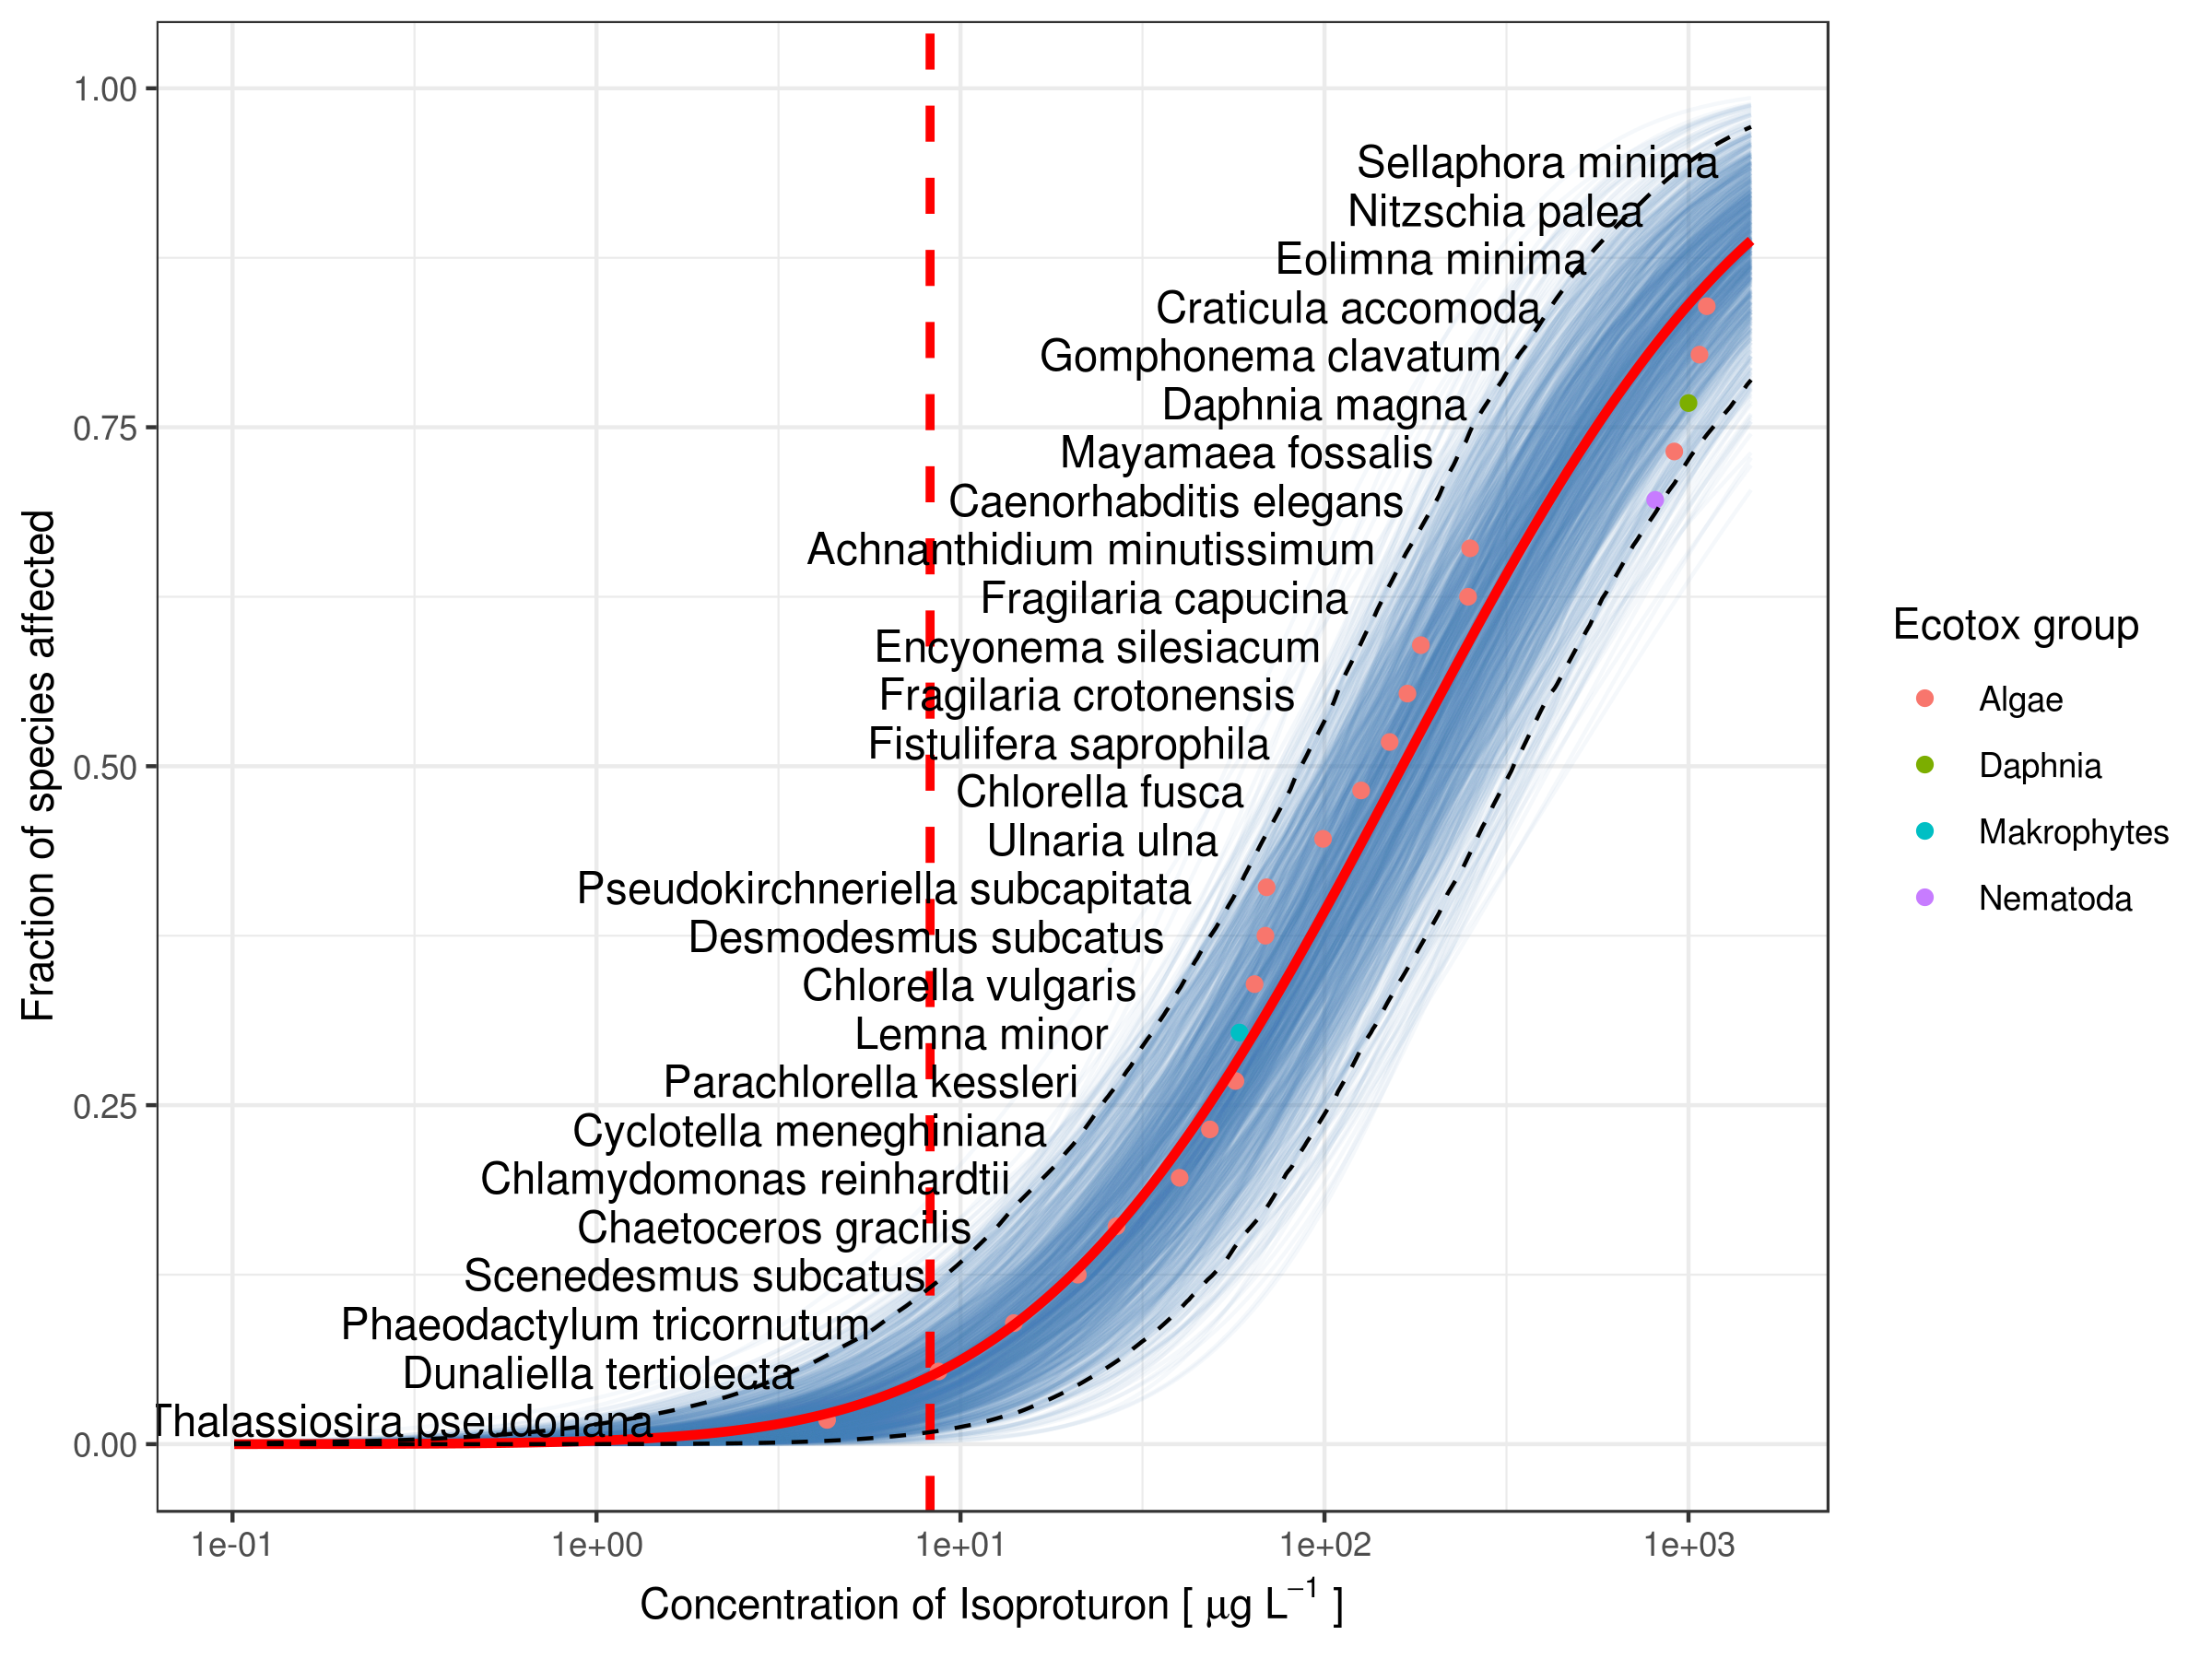
\includegraphics[width=1\linewidth]{article/figures/ssd2_boot.png}
    \caption{SSD plot showing the susceptibility of organisms towards the herbicide Isoproturon. The red line represents the fit and the red dashed line marks the HC\textsubscript{5} value, which is a common measure in CRA. The legend denotes common organism groups used in ecotoxicology.}
    \label{fig:ssd-isoproturon}
\end{figure}


\subsection*{Limitations}
Since the EPA ECOTOX data at hand merely represents a sample of the reality of the toxicity of chemicals on organisms, it has to be stated that the returned Standartox values are subject to change. New studies will be published and constantly incorporated into Standartox, improving the toxicity estimates. However, we expect values of well tested chemical-organism combinations to be relatively stable. A future analysis on the smallest number of tests needed to return trustworthy results, could shed more light on this aspect. Furthermore, toxicity test results are certainly influenced by individual tests parameters, such as pH, temperature or conductivity amongst others \citep{rosenkrantz_influence_2013, li_temperature_2011}. Such information is not included in the aggregation performed by Standartox, since the EPA ECOTOX only provides sparse records on those. Most frequently provided test parameters (and their percentage) are medium temperature (77\%), pH:56\%, hardness:27\%, dissolved oxygen:18\%, Alkalinity:15\% and salinity:9\%. Others are provided for less than 5\% of the tests. A test-mining approach, iterating through the individual test studies could potentially increase this number. However, we argue that using the geometric mean as an aggregate allows for an adequate estimation of the toxicity of a chemical towards an organism group. We prefer the geometric mean in comparison to the arithmetic mean, since it is considerably less influenced by outliers and is suitable for skewed data. Also, the geometric mean is preferable over the median, since the median completely ignores the influence of large or small values, making it unreliable for small data sets <CITATION GEOMETRIC MEAN>.

\subsection*{Other data bases}
Other initiatives tidying the large number of ecotoxicological test results were also developed recently. They partly aim for overlapping goals, yet have limitations or objectives that differentiate them from Standartox. Since 2006, the PPDB provides validated ecotoxicological information on pesticides \citep{lewis_international_2016}.
% TODO lookup NORMAN citation
The Network of reference laboratories, research centres and related organisations for monitoring of emerging environmental substances (NORMAN) focuses on assembling river basin specific pollutants \citep{von_der_ohe_new_2011}. 
Connors et al. \citet{healthandenvironmentalsciencesinstitutehesi_envirotox_2019, connors_creation_2019} published the EnviroTox data base \href{https://envirotoxdatabase.org/} which also uses, amongst others the EPA ECOTOX data as an input. In comparison to Standartox, ENviroTox focuses only on aquatic organisms and uses an qualitative algorithm to exclude unreliable test results. They filter for example the data to fish, amphibian invertebrate and algae taxa, to test durations of above 24 hours and aquatic taxa only and add additional information on toxicity endpoints, such as chronic or acute tests as well as mode of action assignments. In contrast, Standartox doesn't refine to specific test durations, but leaves it up to the user to decide on such parameters. The EnvirTox data base also allows for an aggregation of test results to derive single toxicity values for individual taxa whereas Standartox performs this aggregation for individual chemicals. This has to be done in a cumbersome way by down- and uploading the data manually. Comptox, is a web tool published by the EPA which, similar to Standartox allows for filtering test results and the retrieval of additional chemical information. However, it lacks the possibility to aggregate toxicity test results \citep{usenvironmentalprotectionagency_comptox_2019}. Petschick et al. (in submission) modeled risk threshold level equivalents for aquatic organisms by using ecotoxicological effect data from the EPA ECOTOX. However, none of the above mentioned approaches aim for a standardized aggregation method of toxicity endpoints for individual chemicals. Besides, they also lack the possibility for automated and scriptable user requests for high level programming languages, such as R or Python. Along with newly created ecotoxicological data bases here, methods of how to efficiently store ecotoxicological data are also proposed as can be seen in the MAGIC Knowledge Base \citep{bub_graphing_2019}. This recent increase of efforts to compile ecotoxicological test data bases clearly emphasizes the need for holistic and automated analyses of large-scale ecotoxicological data. Standartox is a tool that puts its focus on the aggregation of toxicity data and by this adds a piece to the puzzle of modern ecotoxicological analyses.

\subsection*{Identify chemicals to be tested}
There is a clear need in ecotoxicology for harmonised approaches to collect ecotoxicological data as other data base compilation attempts recently published show. Hitchock et al. \citet{hitchcock_improving_2018} argue for an increased awareness concerning newly published ecotoxicological test results to facilitate meta analyses across studies. Important statistical parameters, such as mean estimates, variances and sample sizes. Likewise, state variables, including medium temperature, pH, mineral contents or organism age and sex should be reported (if not in the text, in an online repository). Standartox doesn't include such information mainly because the EPA ECOTOX reports only a few of these variables. A future research aim could be to use machine learning techniques to retrieve this information from the referenced articles.
Above all, recent studies showed that, in defiance of many regulation efforts \citep{schafer_future_2019} chemicals can still cause strong adverse effects on organisms and in turn the environment. Neonicotinoids, a group of insecticides was for example related to declines in insectivorous birds \citep{hallmann_declines_2014} and fish yields due to cascading food web effects \citep{yamamuro_neonicotinoids_2019}. Standartox provides means to synthesise ecotoxicological test data, thereby identify research gaps. Furthermore, standardized approaches could potentially reduce unnecessary animal testing by synthesizing existing ecotoxicological test data.

\begin{figure}
    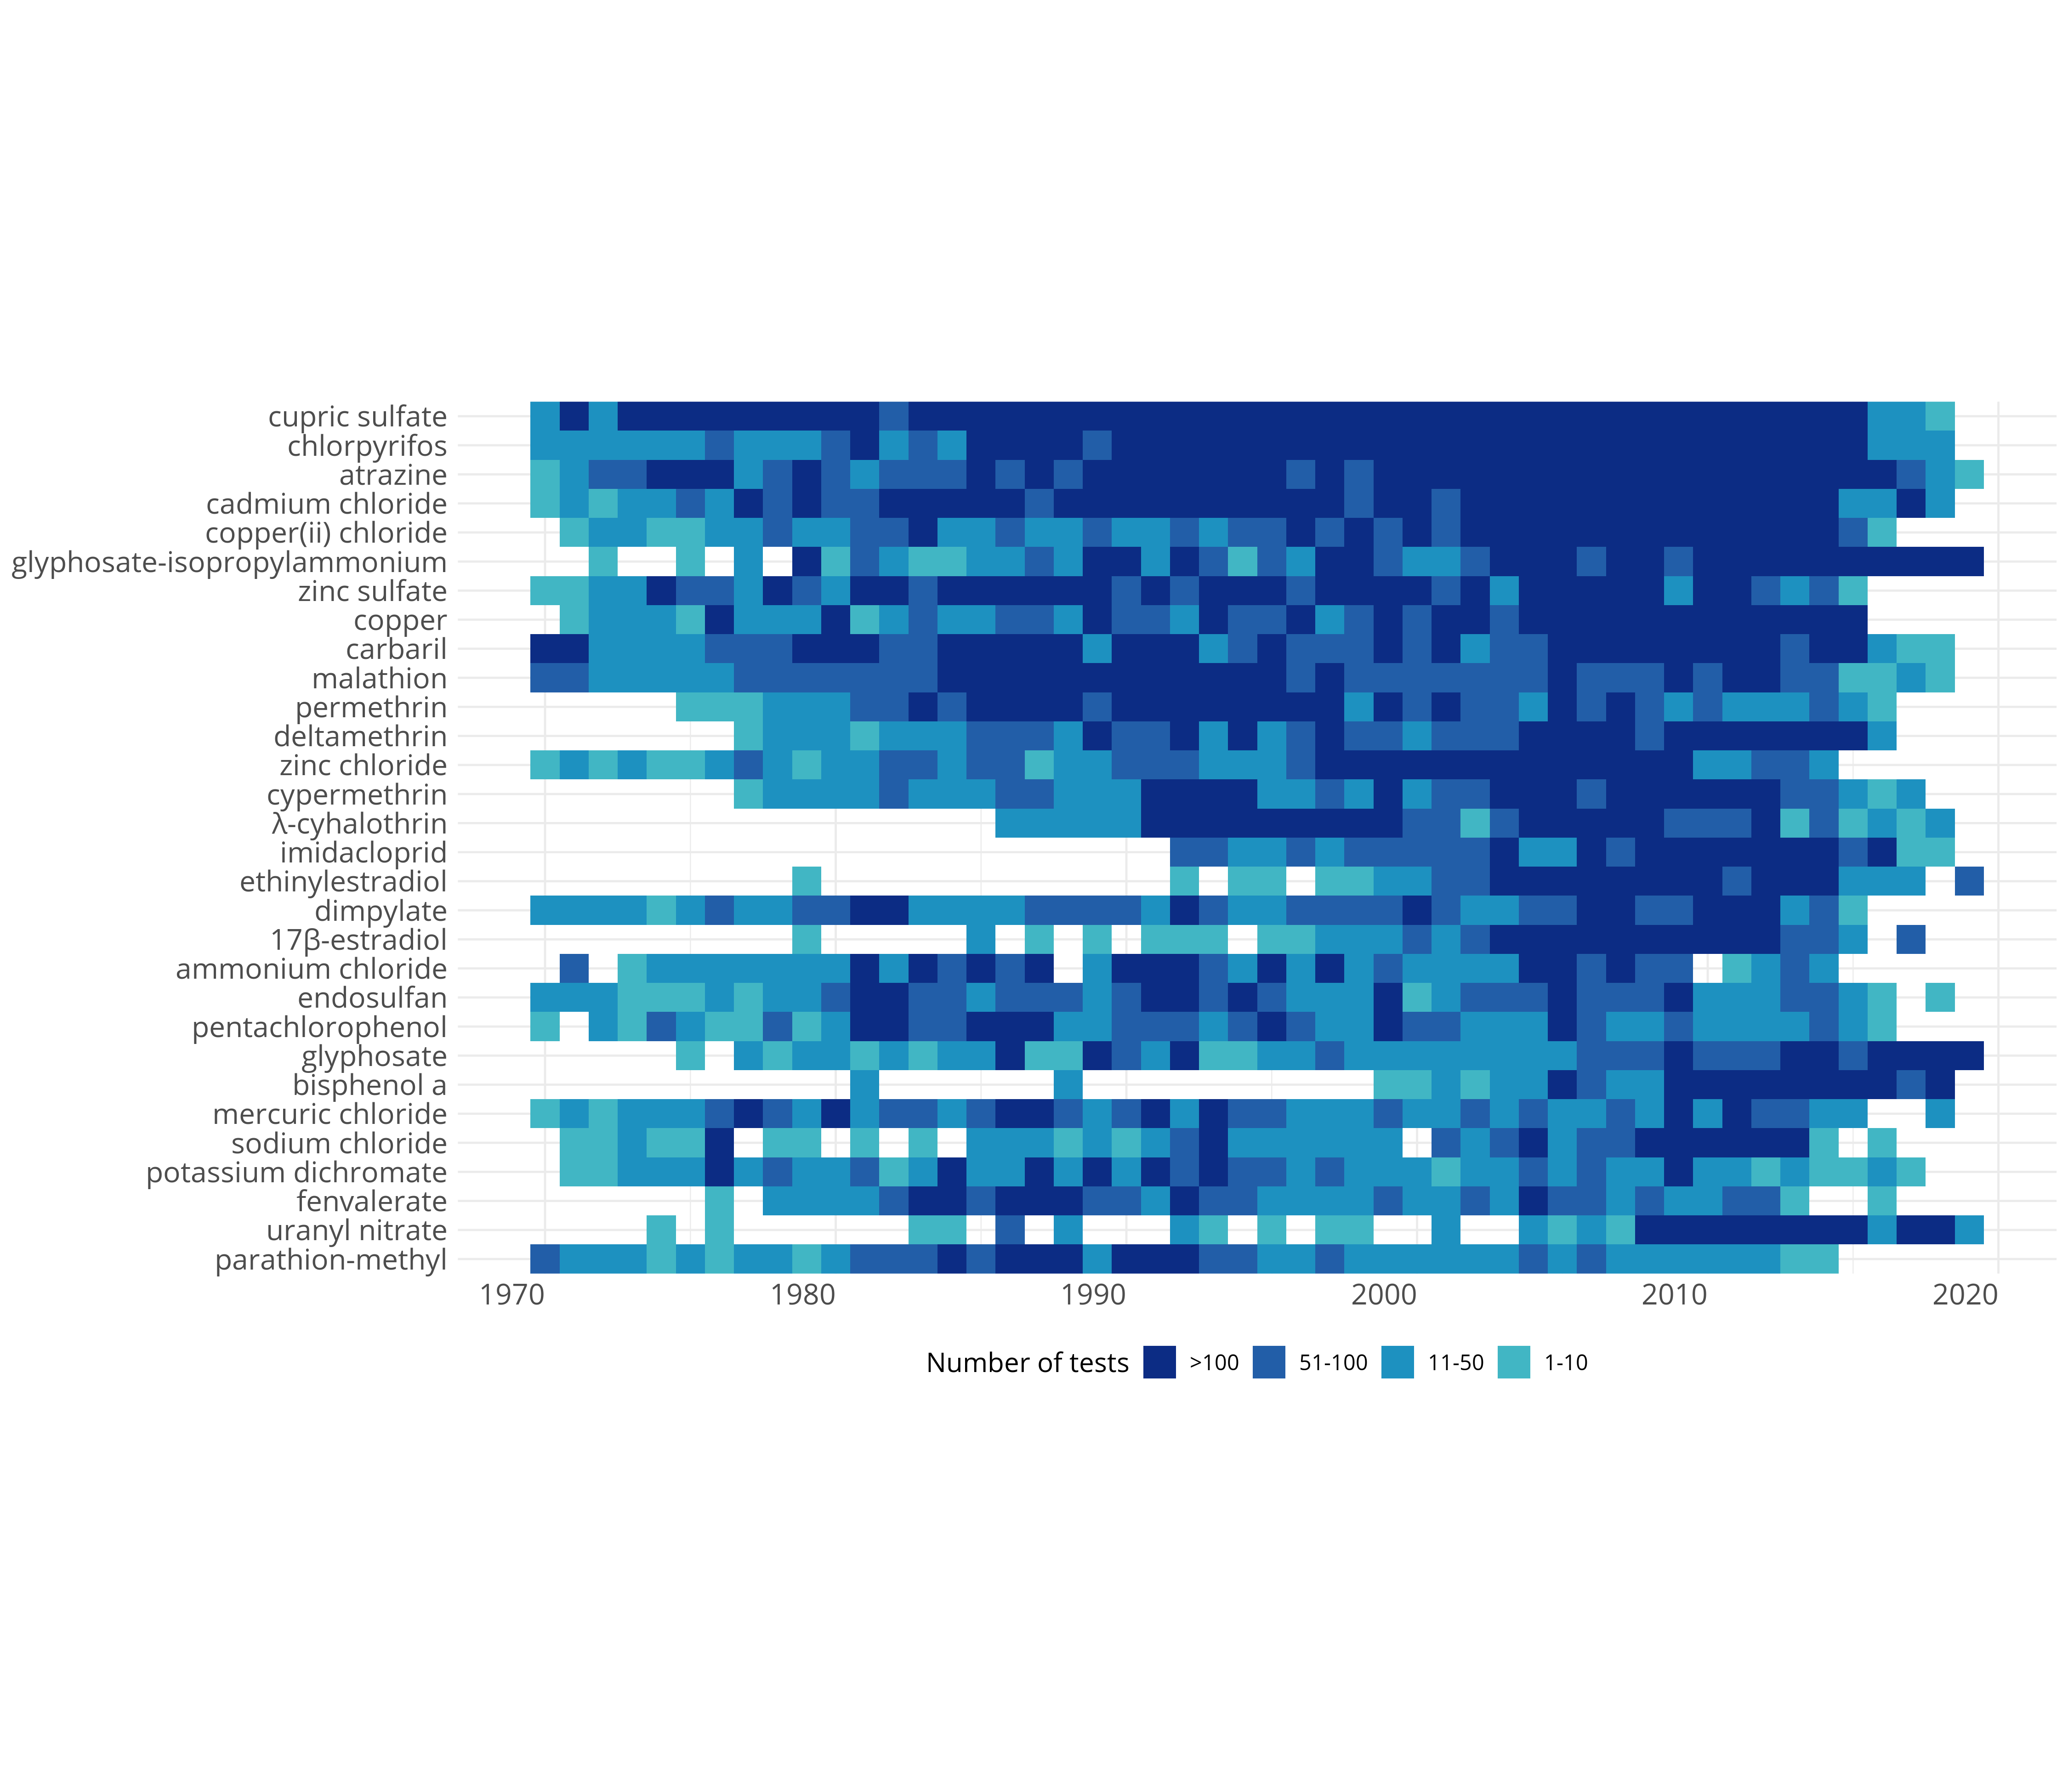
\includegraphics[width=1\linewidth]{article/figures/heatmap_tests_n.png}
    \caption{30 most tested chemicals in EPA ECOTOX.}
    \label{fig:standartox_ppdb_diff}
\end{figure}

%%%%%%%%%%%%%%%%%%%%%%%%%%%%%%%%%%%%%%%%%% TODO %%%%%%%%%%%%%%%%%%%%%%%%%%%%%%%%%%%%%%%%%%
1) \citep{staveley_challenge_2016} describe what is necessary for future ecotoxicology.

%%%%%%%%%%%%%%%%%%%%%%%%%%%%%%%%%%%%%%%%%% OLD %%%%%%%%%%%%%%%%%%%%%%%%%%%%%%%%%%%%%%%%%%%
\iffalse
Besides that, two cleaning steps can also be chosen. Firstly the application allows to exclude test results exhibiting concentrations that are higher than the actual water solubility of the respective chemical at \ang{20} C. Secondly the user can choose to exclude outliers (cf. Table \ref{tab:scripts-app}). The outliers are selected as values that exceed lower (0.25) and the upper (0.75) quartile by 1.5 times the inter-quartile range.
\fi